\documentclass[a4paper,12pt]{report}
\usepackage[margin=1in]{geometry}
\usepackage[T1]{fontenc}
\usepackage[utf8]{inputenc}
\usepackage{lmodern}
\usepackage{microtype}      % subtle font expansion and margin protrusion
\emergencystretch=3em   
\usepackage{tikz}
\usetikzlibrary{calc}
\usepackage{graphicx}
\usepackage{titlesec}
\usepackage{titletoc}              
\usepackage{fancyhdr}
\usepackage{amsmath}
\usepackage{listings}
\usepackage{xcolor}
\usepackage{caption}
\usepackage{subcaption}
\usepackage{array}
\usepackage{multirow}
\usepackage{booktabs}
\usepackage{makecell}
\usepackage{float}
\usepackage{lipsum}
\usepackage{adjustbox}
\usepackage{setspace}
\usepackage{indentfirst}
\setstretch{1.2}
\usepackage[colorlinks=true, linkcolor=black, citecolor=black, urlcolor=black]{hyperref}
\usepackage[backend=biber, style=numeric, sorting=none]{biblatex}
\addbibresource{references.bib}

% vietnamese
\usepackage[T5]{fontenc}
\usepackage[utf8]{inputenc}
\usepackage{lmodern}

\setlength{\headheight}{14.5pt}
\pagestyle{fancy}
\lhead{S\&T Management}
% Right header: "IV. Title" instead of "CHAPTER IV. TITLE", so it no longer overlaps the left header
\renewcommand{\chaptermark}[1]{\markboth{\thechapter.\ #1}{}}

\definecolor{codegreen}{rgb}{0,0.6,0}
\definecolor{codegray}{rgb}{0.5,0.5,0.5}
\definecolor{codepurple}{rgb}{0.58,0,0.82}
\definecolor{backcolour}{rgb}{0.95,0.95,0.92}
\lstdefinestyle{mystyle}{
    backgroundcolor=\color{backcolour},
    commentstyle=\color{codegreen},
    keywordstyle=\color{magenta},
    numberstyle=\tiny\color{codegray},
    stringstyle=\color{codepurple},
    basicstyle=\ttfamily\footnotesize,
    breaklines=true,
    captionpos=b,
    keepspaces=true,
    numbers=left,
    numbersep=5pt,
    showspaces=false,
    showstringspaces=false,
    showtabs=false,
    tabsize=2
}
\lstset{style=mystyle}

% ----- Đánh số kiểu I. / 1. / 2.1. -----
\renewcommand{\thechapter}{\Roman{chapter}}
\renewcommand{\thesection}{\arabic{section}}
\renewcommand{\thesubsection}{\thesection.\arabic{subsection}}

\titleformat{\chapter}[block]
  {\LARGE\bfseries}{\thechapter.}{0.5em}{\MakeUppercase}
\titlespacing*{\chapter}{0pt}{0pt}{1cm}
\titleformat{\section}[block]
  {\large\bfseries}{\thesection.}{0.5em}{}
\titleformat{\subsection}[block]
  {\large\bfseries}{\thesubsection.}{0.5em}{}

% ----- Tiêu đề "TABLE OF CONTENTS" căn giữa -----
\renewcommand{\contentsname}{TABLE OF CONTENTS}
\titleformat{name=\chapter,numberless}[block]
  {\centering\LARGE\bfseries}{}{0pt}{}
\titlespacing*{name=\chapter,numberless}{0pt}{0pt}{1.5cm}

% ----- Định dạng các dòng trong mục lục -----
\titlecontents{chapter}[0pt]
  {\addvspace{10pt}\bfseries}
  {\thecontentslabel.\ \MakeUppercase}
  {\MakeUppercase}
  {\hfill\contentspage}
\titlecontents{section}[1.5em]
  {\addvspace{2pt}}
  {\thecontentslabel.\ }
  {}
  {\hfill\contentspage}
\titlecontents{subsection}[3em]
  {\addvspace{2pt}}
  {\thecontentslabel.\ }
  {}
  {\hfill\contentspage}


\begin{document}

% ===================== TRANG BÌA =====================
\thispagestyle{empty}

\begin{tikzpicture}[remember picture, overlay]
    \draw[line width=2pt]
        ($(current page.south west) + (0.5in, 0.5in)$)
        rectangle
        ($(current page.north east) - (0.5in, 0.5in)$);
\end{tikzpicture}

\begin{center}
    {\Large \textbf{University of Science and Technology of Hanoi}}\\[0.5cm]

    
\includegraphics[width=0.5\textwidth]{images/usth.png}\\[1cm]

    {\LARGE \textbf{Science and Technology Management}}\\[1cm]

    \rule{\textwidth}{0.75pt}\\[0.5cm]
    {\LARGE \textbf{Analysis of a company's technology management activities}}\\[0.5cm]
    \rule{\textwidth}{0.75pt}\\[1.0cm]
\end{center}

% ----- Danh sách thành viên -----
\begin{center}
    \large
    \renewcommand{\arraystretch}{1.1}
    \begin{tabular}{l@{\hspace{1.75cm}}r}
        \multicolumn{2}{l}{\hspace{-1.2cm}\textbf{\Large Members:}} \\[0.3cm]
        \textbf{Nguyen Huy Hai} & 2640088\\
        \textbf{Dang Trung Hieu} & 2640076\\
        \textbf{Pham Mai Hanh} & 2640013\\
        \textbf{Luyen Pham Ngoc Khanh} & 2640014\\
        \textbf{Vuong Hong Minh} & 2640110\\
        \textbf{Trinh Quang Minh} & 2640018\\
        \textbf{Nguyen The Anh} & 2640003\\
        \textbf{Nguyen Thi Minh Anh} & 2640059\\
        \textbf{Nguyen Nam Anh } & 2640058
    \end{tabular}
\end{center}

\vfill
\begin{center}
    \textit{Hanoi, Nov 2026}
\end{center}
\newpage


% ===================== TABLE OF CONTENTS =====================
% \setcounter{page}{2}
\tableofcontents
\listoffigures
% Marks a source that has no entry in references.bib yet.
\providecommand{\pending}[1]{\textbf{[#1]}}

% ===================== MAIN CONTENT =====================
% Source-tracking convention:
%   % NOTE: ...                    -> needs a decision/check by the authors
% "PDF" below = sources/FPT Technology Management.pdf
% "slides" below = sources/SciTech-Group 2-Sunday.pptx.pdf
% Citation keys S1--S29 = the [S1]--[S29] source list on PDF p.6.

% -------------------------------------------------
% CHAPTER I
% Responsible: Hai
% executive summary and 1. Company background and the AI-First shift
% -------------------------------------------------
\chapter{Introduction}

FPT Corporation, Vietnam's largest IT services group, has repositioned itself as an ``AI-First'' company. 
We analyse this shift with Gregory's (1995) technology management process -- identification, selection, acquisition, 
exploitation and protection -- and assess FPT's technological capability with the THIO model. FPT's approach is consistent 
across the process: it builds AI infrastructure, platforms and delivery capability on top of chips and models supplied by 
partners, rather than developing frontier foundation models of its own. It acquired compute through a strategic partnership 
with NVIDIA, shared the investment in Japan with Sumitomo and SBI Holdings, and partners with OpenAI and NAVER Cloud for models 
\cite{S5,S6,S8,S9}.

Results are measurable but early. AI and data analytics revenue reached VND~2,915bn in the first nine months of 2026, up 55\%, 
against 12.4\% growth for the group \cite{S2}. Both AI Factories passed 90\% utilisation and turned profitable in Q2 2026, 
according to FPT \cite{S4}. However, AI and data is only about 7.3\% of group revenue, and FPT does not disclose AI margins or 
return on investment \cite{S2}. Our judgement: the strategy is coherent and operationally on track, but its financial payoff is 
not yet proven, and FPT's advantage lies in customers, delivery scale and know-how rather than in ownership of core AI technology.

% -------------------------------------------------
\chapter{Company background and the AI-First shift}
FPT was founded in 1988 and operates in technology (global and domestic IT services), telecommunications, and education. 
Its traditional outsourcing model earns revenue in proportion to the number of engineers and hours delivered. 
Generative AI threatens that model, because clients expect faster and cheaper delivery, but it also creates demand for 
AI consulting, integration and infrastructure. FPT's 2025 annual report describes AI as a core capability of its growth 
strategy \cite{S16}.

An accounting change matters for every 2026 comparison: from 2026 FPT accounts for FPT Telecom by the equity method instead 
of full consolidation. Reported 2026 revenue is therefore smaller and cannot be compared directly with FY2025; FPT reports 
growth on a restated basis. On this basis, 9M2026 revenue was VND~40,023bn (+12.4\%) and profit before tax VND~8,770bn (+17\%) 
\cite{S2}.


% -------------------------------------------------
\chapter{Technology Identification}

Identification means finding and assessing technologies that are, or may become, important to the business, through 
technology assessment, market scanning and information management (Gregory, 1995). Four signals pointed FPT toward AI:

\begin{itemize}
  \item \textbf{Market.} Gartner forecast worldwide AI spending of nearly US\$1.5 trillion in 2025 and more than US\$2 trillion in 2026 \cite{S1}.
  \item \textbf{Clients.} Enterprises are moving from AI pilots to company-wide, platform-driven deployment \cite{S17}.
  \item \textbf{Competition.} AI coding tools reduce the effort needed for software work, putting pressure on outsourcing sold by man-hours (our analysis).
  \item \textbf{Policy.} Vietnam lists AI among its national strategic technologies (Decision 21/2026/QĐ-TTg), and Japan is building sovereign AI capacity, which FPT's Japanese partnership is intended to support \cite{S6}.
\end{itemize}

FPT therefore identified AI as both a threat to its headcount-based model and an opportunity in consulting, integration 
and infrastructure.
FPT's response was an AI-First strategy, with AI as a core capability.

\section{Strategic implications for FPT}
The four signals produced three linked implications for FPT's technology strategy.

\begin{table}[H]
\centering
\caption{Strategic implications of AI identification for FPT}
\label{tab:ai-identification}
\begin{tabular}{p{0.19\textwidth} p{0.72\textwidth}}
\toprule
\textbf{Dimension} & \textbf{Implication} \\
\midrule
Threat & AI may reduce demand for headcount-based outsourcing and billable man-hours. \\
Opportunity & FPT can expand into AI consulting, system integration, enterprise applications and the infrastructure required to run them. \\
Response & FPT's AI-First strategy positions AI as a core capability, combining existing models with FPT's platform and integration capabilities. \\
\bottomrule
\end{tabular}
\end{table}

Taken together, these drivers explain why FPT treats AI Factory infrastructure, enterprise platforms and AI-enabled services as strategic priorities. The AI-First response seeks to convert pressure on the traditional delivery model into higher-value consulting, integration and infrastructure services.


% -------------------------------------------------
% Technology Selection and Acquisition
% PDF section 3
% -------------------------------------------------
\chapter{Technology Selection}

Selection methods include scenario analysis, portfolio analysis (SWOT, BCG), multi-criteria decision making (MCDM), 
expert judgment and financial analysis. FPT's decision was a choice between discrete alternatives, which fits multi-attribute 
decision making (MADM). FPT does not publish its selection method, so the comparison below is our qualitative analysis.

\begin{table}[htbp]
  \centering
  \small
  \caption{Develop own frontier model vs.\ build on top of existing models}
  \label{tab:selection}
  \begin{tabular}{>{\raggedright\arraybackslash}p{2.4cm}>{\raggedright\arraybackslash}p{5.9cm}>{\raggedright\arraybackslash}p{5.9cm}}
    \toprule
    \textbf{Criteria} & \textbf{Develop own frontier model} & \textbf{Build on top of existing models} \\
    \midrule
    Strategic fit & Far from FPT's core IT services & Uses FPT's clients and delivery teams \\ \addlinespace
    Feasibility & Huge compute and scarce research talent & NVIDIA GPUs; partner and open models \\ \addlinespace
    Investment & Mistral AI raised \texteuro1.7bn (2025) and \texteuro3bn (2026) \cite{S20,S21} & About US\$200m per AI Factory site \cite{S5,S7} \\ \addlinespace
    Decision & Not selected & Selected \\
    \bottomrule
  \end{tabular}
\end{table}
% NOTE: "About US$200m per AI Factory site" (p.2, also slide 5 "~US$200m per site") vs p.2 section 4 / p.5 Key figures "US$200m plan for an AI Factory" -- unclear whether US$200m is per site or one plan in total.

\section{Selected technology priorities}

FPT selected four priorities:
\begin{itemize}
    \item \textbf{AI Factory.} GPU infrastructure for training and running enterprise AI services.

    \item \textbf{FleziPT.} An AI delivery platform launched in August 2025 \cite{S18}.

    \item \textbf{FPT.AI.} AI agents and related enterprise applications.

    \item \textbf{Partner and open models.} Integration of models supplied through partners and open-model ecosystems, allowing FPT to focus on application and delivery capabilities.
\end{itemize}

Semiconductors are kept as a longer-term option:
on 30 December 2025 FPT delivered its first commercial batch of power-management ICs to a Japanese electronics company
through the distributor Restar \cite{S19}.


% -------------------------------------------------
% PDF section 4
% -------------------------------------------------
\chapter{Technology Acquisition}

A firm can acquire a selected technology by making it (in-house R\&D),
buying it (purchasing, outsourcing, licensing, M\&A) or collaborating
with partners. FPT uses all three routes, but collaboration dominates.

\begin{itemize}
    \item \textbf{Collaborate.} On 23 April 2024 FPT signed a comprehensive
    strategic partnership with NVIDIA and announced a US\$200m plan for
    an AI Factory \cite{S5}. In April 2025 Sumitomo Corporation and SBI
    Holdings each agreed to take 20\% of FPT Smart Cloud Japan, which
    runs the Japanese AI Factory, while FPT keeps 60\% \cite{S6}.
    In 2026 FPT became an OpenAI Select Partner (August) and signed an
    MoU with NAVER Cloud covering AI Factory projects, GPU-as-a-Service
    and access to HyperCLOVA X (October) \cite{S8,S9}.

    \item \textbf{Buy.} FPT purchases NVIDIA GPUs (H100, H200 and,
    from 2026, HGX B300) \cite{S7,S10}. It acquired NAC, a Japanese IT
    firm with about 300 engineers, in March 2024 -- its first acquisition
    in Japan \cite{S11} -- and David Lamm Consulting, a German energy-sector
    IT consultancy, in May 2025 \cite{S12}.

    The acquisitions involve two methods:
    \begin{itemize}
        \item \textbf{Purchasing:} NVIDIA GPUs.
        \item \textbf{M\&A:} NAC and David Lamm Consulting.
    \end{itemize}

    \item \textbf{Make.} FPT designs and operates the AI Factories itself,
    built the FleziPT platform, holds patents from in-house R\&D, and
    designs its own power-management chips \cite{S13,S14,S19}.
    The patents from in-house R\&D are held in the US and Taiwan.
\end{itemize}

\textbf{Reasons to collaborating:} As in the Pfizer--BioNTech case, collaboration shares risk, combines complementary capabilities (FPT's engineering with the Japanese partners' client networks) and speeds up market entry. The trade-off is dependence on NVIDIA as the key GPU supplier.

\section{Case study: AI Factory}

\begin{table}[htbp]
  \centering
  \small
  \caption{AI Factory milestones}
  \label{tab:aifactory}
  \begin{tabular}{>{\raggedright\arraybackslash}p{1.4cm}>{\raggedright\arraybackslash}p{13.0cm}}
    \toprule
    \textbf{Year} & \textbf{Milestone} \\
    \midrule
    2024 & NVIDIA partnership (April); AI Factory launched in Japan with NVIDIA H200 (13 November) and in Vietnam with H100 (November) \cite{S5,S7} \\ \addlinespace
    2025 & Sumitomo and SBI take 40\% of the Japan unit (April); TOP500 list (June): Japan \#36 (49.85 PFLOPS), Vietnam \#38 (46.65 PFLOPS) \cite{S6,S10} \\ \addlinespace
    2026 & NVIDIA HGX B300 announced (March); Vietnam site at breakeven and Japan site loss-making, average utilisation about 60\% (February); both sites above 90\% utilisation and profitable (Q2) \cite{S3,S4} \\
    \bottomrule
  \end{tabular}
\end{table}

Analysts estimate AI Factory revenue at about US\$12m in H1 2026 \cite{S4}. FPT does not publish a separate profit and loss for each site, so profitability rests on company disclosure.

% TODO: where is the fig
\begin{figure}[htbp]
  \centering
  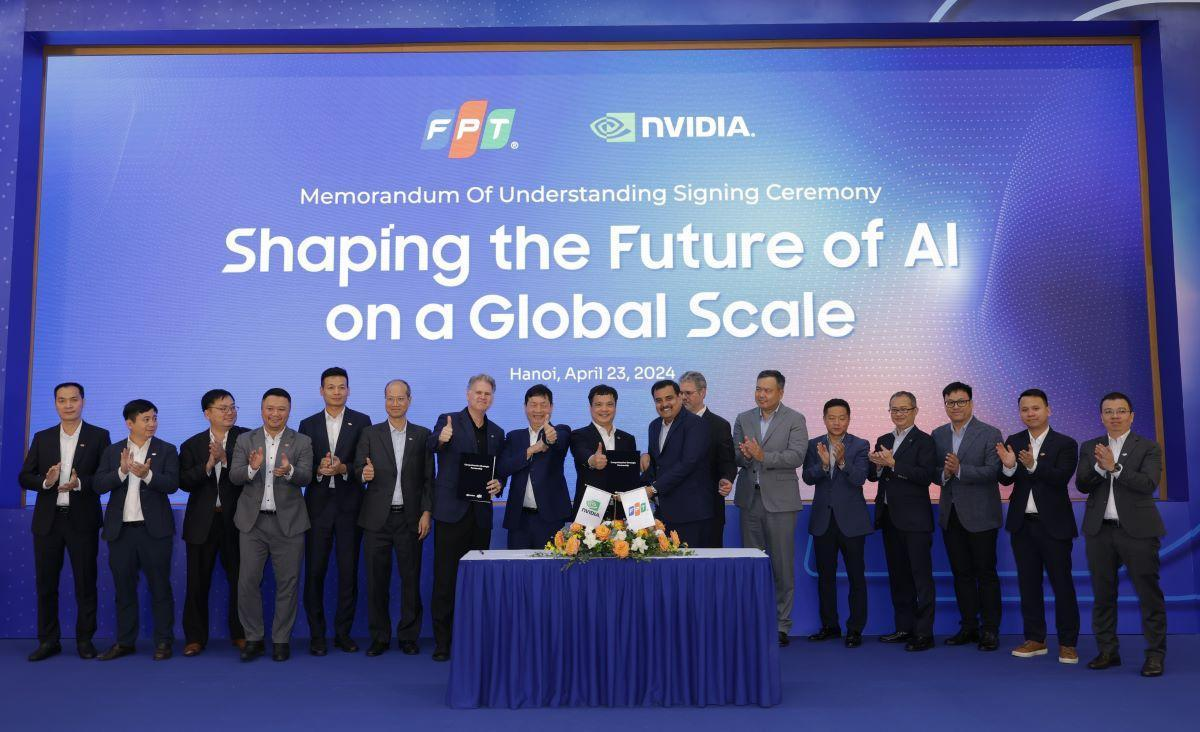
\includegraphics[width=0.75\textwidth]{images/fpt_nvidia_signing.jpg}
  \caption{FPT--NVIDIA signing, Hanoi, April 2024}
  \label{fig:nvidia-signing}
\end{figure}

% -------------------------------------------------
% PDF section 5: Technological Capability
% -------------------------------------------------
\chapter{Technological Capability}

The THIO model (Technology Atlas; Sharif) describes technology as four components: technoware, humanware, infoware and orgaware.

\begin{table}[htbp]
  \centering
  \small
  \caption{THIO components: FPT evidence}
  \label{tab:thio}
  \begin{tabular}{>{\raggedright\arraybackslash}p{2.6cm}>{\raggedright\arraybackslash}p{11.8cm}}
    \toprule
    \textbf{Component} & \textbf{FPT evidence} \\
    \midrule
    Technoware & AI Factories with NVIDIA H100/H200 GPUs, B300 from 2026; TOP500 \#36 and \#38 (June 2025) \cite{S7,S10} \\ \addlinespace
    Humanware & Partnership with Mila (Quebec AI Institute) since June 2020, renewed 2023; AI research hub in Quy Nhon \cite{S15} \\ \addlinespace
    Infoware & FleziPT delivery platform; patents for AI4Code, SoundAI and Akabot \cite{S13,S14,S18} \\ \addlinespace
    Orgaware & CASAN five-level AI maturity framework; ISO/IEC 42001 certified AI management system \cite{S22,S23} \\
    \bottomrule
  \end{tabular}
\end{table}

We do not compute a technology contribution coefficient (TCC), because public data does not support reliable 0--1 ratings for each component. Using UNIDO's capability categories, our assessment is that FPT is strong in acquisitive and operative capability -- it runs two AI Factories above 90\% utilisation -- while its innovative capability is applied: it patents applications but does not develop its own foundation models.



% -------------------------------------------------
% CHAPTER Technology Exploitation 
% -------------------------------------------------
\chapter{Technology Exploitation}

A technology creates value only when customers adopt and pay for it. FPT earns from AI in three ways, summarised in 
Table~\ref{tab:channels}.
% NOTE: existing text, not found in the PDF. The PDF (p.3) classifies exploitation as in-house development / joint commercialisation / selling technology (written below), not as the three channels of Table~\ref{tab:channels}. The claim "creates value only when customers adopt and pay for it" is also not in the PDF.

Technology can be exploited through in-house development, joint commercialisation or selling technology.

\textbf{In-house development (main route).} In September 2025 FPT signed a five-year, US\$256m contract -- its largest to date -- to deliver AI-augmented digital transformation services to an unnamed Asian energy company \cite{S24}. In May--June 2026 it signed six AI transformation MoUs in Thailand and Singapore, with UOB, SCG, SATS, ComfortDelGro, CPF and Sembcorp \cite{S25}. The FPT.AI platform serves more than 200 enterprise clients \cite{S26}.

\textbf{Joint commercialisation.} The Japanese AI Factory is co-owned with Sumitomo and SBI, giving access to their client networks \cite{S6}. The NAVER Cloud MoU covers joint AI Factory and GPU-as-a-Service business \cite{S9}.

\textbf{Selling technology.} We found no public evidence that FPT licenses or sells its AI technology.

\section{Three commercialisation channels}
% NOTE: existing section, heading not in the PDF. The whole section (table + three paragraphs) uses a classification that is not in the PDF and cites keys outside the PDF source list (A22, A26, A27, M6). Details per paragraph below.

\begin{table}[htbp]
  \centering
  \small
  \caption{How FPT earns from AI}
  \label{tab:channels}
  \begin{tabular}{>{\raggedright\arraybackslash}p{2.8cm}>{\raggedright\arraybackslash}p{4.6cm}>{\raggedright\arraybackslash}p{6.4cm}}
    \toprule
    \textbf{Channel} & \textbf{What clients pay for} & \textbf{Real-world example} \\
    \midrule
    AI transformation projects & Design and build of AI systems across a client's business & Contract worth tens of millions of US dollars with a global materials group (April 2026) \cite{S25} \\ \addlinespace
    AI agents & Ready-made AI agents for uses such as customer service, sales and document processing & 10,220 FPT.AI agents deployed (2025) \cite{A26} \\ \addlinespace
    GPU cloud & Rented computing capacity for training and running AI models & Analysts report that AI Factory clients are mainly banks and technology companies \cite{M6} \\
    \bottomrule
  \end{tabular}
\end{table}
% NOTE: existing table, not found in the PDF: the three channels, "what clients pay for", the materials-group contract (April 2026), 10,220 agents, and "clients mainly banks and technology companies" are not in the PDF. Also, row 1 cites S25 (six partnerships in Thailand/Singapore) while the paragraph below cites A22 for the same contract.

\textbf{AI transformation projects:} In April 2026, FPT signed a contract worth tens of millions of US dollars with a global materials group to move the group toward an agentic AI operating model on FleziPT \cite{A22}. In May 2026, it announced 6 AI transformation partnerships in Thailand and Singapore, with partners including UOB, SCG, SATS and ComfortDelGro; these include memoranda of understanding and are not described as paid contracts \cite{S25}. In 2025, it signed a record USD~256~million AI-powered digital solutions contract with an energy company \cite{A27}.
% NOTE: not in the PDF: the April 2026 materials-group contract and "agentic AI operating model on FleziPT"; "not described as paid contracts". PDF says "May--June 2026" and "MoUs" (also lists CPF and Sembcorp), and dates the US$256m contract September 2025, five-year, cited [S24] (here cited A27). Duplicates the "In-house development" paragraph above.

\textbf{AI agents:} In 2025, FPT.AI reported 10,220 AI agents deployed in business operations and more than 200 customers in 15 countries. Separately, FPT's language models processed 169 million requests \cite{A26}. Typical uses include customer service, sales support and document processing.
% NOTE: not in the PDF: 10,220 agents, 15 countries, 169 million requests, typical uses.

\textbf{GPU cloud:} Companies rent AI Factory capacity to train or run their own models. Analysts report that these clients are mainly banks and technology companies \cite{M6}.
% NOTE: not found in the PDF section 6. The PDF only touches on this in section 9 (p.5, "Is the AI Factory just GPU rental? Partly. ..."); "clients are mainly banks and technology companies" is not in the PDF.

\section{Financial results}
% NOTE: existing heading; the corresponding PDF heading (p.4) is "Commercialisation results".

AI and data analytics revenue was VND~2,612 billion in 2025 (+40.7\%), equivalent to about USD~100~million and 15.5\% of digital-transformation revenue \cite{M1,M6}. It reached VND~1,842 billion in H1 2026 (+54\%) and VND~2,915 billion in 9M2026 (+55\%), about 7.3\% of group revenue (our calculation: 2,915 / 40,023) \cite{M14,S2}.
% NOTE: not in the PDF: +40.7% for 2025, "about USD 100 million", "15.5% of digital-transformation revenue", H1 2026 VND 1,842bn (+54%). The PDF cites only [S2] for these figures.

At foreign level, FPT won 16 projects worth more than USD~10~million each in 9M2026, down from 19 a year earlier, while the number of contracts of at least USD~1~million rose 29\% to 163 \cite{M15}. In 2025, newly signed AI and cloud revenue was VND~1,540 billion, and recognised revenue was VND~913 billion (+48.4\%) \cite{S16}.
% NOTE: existing paragraph, not found in the PDF (16 / 19 projects > USD 10m, 163 contracts >= USD 1m, VND 1,540bn signed and VND 913bn recognised AI and cloud revenue).

These figures should be interpreted with caution. Adoption figures such as agents, requests show usage, not profit. Judging commercial success requires revenue, margin and client retention data, and FPT discloses only part of this.
% NOTE: "agents, requests" and "client retention data" are not in the PDF.

The 9M2026 figure is already above the full-year 2025 figure. Its 55\% growth is about four times the group's 12.4\% growth \cite{S2}. Growth and utilisation are proven; profitability is not, because FPT does not disclose AI margins or return on investment.




% -------------------------------------------------
% CHAPTER IV - Technology Protection
% Responsible: Minh
% at 6. Technology protection
% -------------------------------------------------
\chapter{Technology Protection}
Protection means keeping control of the value a technology creates. For FPT, this has three parts: intellectual property, certified governance and regulatory compliance.
% NOTE: existing text, not found in the PDF. The PDF (p.4) defines protection differently (next paragraph) and does not split it into these three parts.

Protection management covers identifying own and shared technology assets, managing the IP portfolio, managing knowledge workers' IP, and managing IP in collaborations.

\section{Intellectual property}
% NOTE: existing heading, not in the PDF. It covers the PDF run-in parts "Own and shared assets", "Patent portfolio" and "IP in collaborations" (p.4).

FPT protects its intellectual property through the patents described in Chapter~II, through proprietary platform know-how, and through contracts with clients and partners. Because the base models belong to OpenAI, NAVER or open-source projects, FPT's patents protect only its own application layers. In practice, process know-how and client relationships are more important protections.
% NOTE: "patents described in Chapter~II" -- Chapter II is now "Company background"; the patents are described below (PDF p.4) and in Chapter "Technological Capability". "contracts with clients and partners" and "process know-how and client relationships are more important protections" are not in the PDF (p.5 only says FPT "keeps delivery know-how in-house").

\textbf{Own and shared assets.} FPT's own assets include FleziPT, AI4Code, Akabot and its chip designs. Shared or external assets include NVIDIA GPUs and the models of OpenAI and NAVER.

\textbf{Patent portfolio.} FPT obtained a US patent for a neural network system that generates and ranks source code, used in AI4Code, describing itself as the first Vietnamese company with such a patent (2025) \cite{S13}. It received a US patent for SoundAI acoustic anomaly detection (November 2025) \cite{S13} and patents for Akabot's document classification in the US (2023) and Taiwan (2026); Akabot serves nearly 2,000 customers \cite{S14}.
% NOTE: the AI4Code patent is cited to [S13], whose title is about the SoundAI acoustic anomaly detection patent; please check the source for AI4Code.

\section{Certified governance}
% NOTE: existing heading, not in the PDF. It corresponds to the PDF run-in part "Security and compliance" (p.4).

FPT's governance is evidenced by external certification:

\begin{itemize}
  \item \textbf{ISO/IEC 42001 (AI management).} FPT Software was the first Vietnamese company to receive accredited certification for ISO/IEC 42001, the international standard for AI management systems \cite{S23,M11}. The certification for its AI management system was received in January 2026 \cite{S23}.
  % NOTE: "FPT Software" and "first Vietnamese company" are not in the PDF (PDF says "FPT").
  \item \textbf{SOC~2 and SOC~3 (cloud security).} The Vietnam AI Factory holds SOC~2 Type~II and SOC~3 reports, while the Japan site holds a SOC~2 Type~I report \cite{S28}.
  \item \textbf{HITRUST AI Security (AI security).} In February 2026, FPT's Hanoi data centre received HITRUST r2 certification, including the HITRUST AI Security Certification, which covers threats such as data poisoning, model inversion and prompt injection \cite{M18}.
  % NOTE: "covers threats such as data poisoning, model inversion and prompt injection" is not in the PDF; the PDF cites [S27] (here M18).
\end{itemize}

\section{Regulatory compliance: Vietnam's AI Law}
% NOTE: existing heading, not in the PDF; content corresponds to the last sentence of "Security and compliance" (p.4).

Regulation is now a formal constraint. Vietnam's Law on Artificial Intelligence (No.~134/2025/QH15) was passed on 10~December 2025 with 429 of 434 votes and took effect on 1~March 2026 \cite{M19}. The law:

\begin{itemize}
  \item classifies AI systems into three risk tiers;
  \item requires conformity assessment for high-risk systems;
  \item requires important AI applications in essential sectors to run on national AI infrastructure;
  \item gives existing systems in the medical, education and financial sectors 18 months to comply \cite{M20}.
\end{itemize}
% NOTE: not in the PDF: "429 of 434 votes", item 3 (national AI infrastructure) and item 4 (18 months for medical, education and financial sectors). The PDF cites [S29] (here M19, M20).

The law adds compliance costs to FPT's banking and healthcare work. At the same time, its emphasis on local infrastructure could favour domestic providers; this second point is our interpretation, not a benefit stated by FPT.
% NOTE: not found in the PDF section 7. The closest source text is p.5 (section 9): the AI Law "adds compliance cost for high-risk systems, but FPT is already prepared with ISO/IEC 42001 and HITRUST AI certification". "banking and healthcare" and "could favour domestic providers" are not in the PDF.

\section{Key risks and management responses}
% NOTE: existing heading, not in the PDF; corresponds to the PDF run-in part "Risks to manage (our analysis)" (p.4). The PDF gives no management responses.

Table~\ref{tab:risks} sets out the key risks identified in our analysis, together with possible management responses. These are analytical risks, not failures that FPT has reported.
% NOTE: "possible management responses" are not in the PDF.

\begin{table}[htbp]
  \centering
  \small
  \caption{Key risks and possible management responses}
  \label{tab:risks}
  \begin{tabular}{>{\raggedright\arraybackslash}p{2.8cm}>{\raggedright\arraybackslash}p{6.4cm}>{\raggedright\arraybackslash}p{4.6cm}}
    \toprule
    \textbf{Risk} & \textbf{Description} & \textbf{Possible response} \\
    \midrule
    Idle GPUs & GPU costs and idle capacity if demand weakens & Utilisation dashboards and pre-sold capacity \\ \addlinespace
    Dependence on key suppliers & Dependence on NVIDIA for chips, and on OpenAI and NAVER for models & Multi-vendor and multi-model architecture \\ \addlinespace
    AI errors and privacy & Model errors and data privacy incidents at clients & Human review, audit logs and systematic model evaluation \\ \addlinespace
    Fewer billable hours & Revenue cannibalisation, as faster AI delivery reduces billable effort & Outcome-based pricing \\
    \bottomrule
  \end{tabular}
\end{table}
% NOTE: not in the PDF: the whole "Possible response" column; "GPU costs", "at clients", "revenue cannibalisation"; the PDF says "model suppliers" without naming OpenAI and NAVER.


% -------------------------------------------------
% CHAPTER VI - CONCLUSION
% Responsible: Khanh
% at 8. Conclusion
% ------------------------------------------------
\chapter{Conclusion}

Gregory's five processes explain the logic of FPT's strategy. In identification and selection, AI posed a threat to billable software work while creating demand for enterprise automation. FPT chose to build solutions on existing models and acquired much of the necessary capability through collaboration \cite{A8,A13,A16}. It exploits that capability mainly through its own delivery teams, supplemented by joint commercialisation. Revenue in the reported AI and analytics category is growing rapidly but still makes up a small share of group sales \pending{FPT 9M2026 results}. Protection centres on what FPT develops: proprietary platforms, implementation know-how and granted patents for applications such as acoustic anomaly detection \cite{S13}. Its certified management system supports oversight, while NVIDIA GPUs and third-party models remain external technologies on which delivery depends \cite{S23,A21,A7}.
  % NOTE: "creating demand for enterprise automation" -- the PDF names the opportunity as AI consulting, integration and infrastructure (p.1--2). "Its certified management system supports oversight" is not in the PDF conclusion. \pending{FPT 9M2026 results} corresponds to [S2]; A8, A13, A16, A21, A7 are outside the PDF source list.

Existing customer relationships help FPT identify work worth automating. Its delivery scale lets it serve clients across markets, and its technical and industry knowledge helps teams adapt models to specific workflows. These advantages support a coherent strategy and credible operational progress. The financial payoff remains open. Future assessments should track AI operating margins and ROI, exposure to GPU and model suppliers, and AI's share of group revenue under a consistent definition.
% NOTE: not in the PDF: the first two sentences (customer relationships help identify work worth automating; delivery scale serves clients across markets; industry knowledge adapts models to workflows) and "under a consistent definition".

FPT's competitive advantage rests on customers, delivery scale and know-how rather than on owning core AI technology.


% ===================== REFERENCES =====================
\chapter*{References}
\addcontentsline{toc}{chapter}{References}
\printbibliography[heading=none]

\end{document}